\section{Object and Event Selection} 
\label{sec:llvv_selection}

To successfully separate the scarce signal events from the overwhelming particle multiplicity generated during proton--proton collisions, researchers must deploy a highly rigorous extraction protocol targeting specific final-state objects. This workflow initiates with the raw electronic impulses captured by the ATLAS detector, translating them into reconstructed physical entities—namely jets, muons, and electrons. An extensive breakdown of this ATLAS object reconstruction methodology is provided in Chapter~\ref{chap:recon}. Once reconstructed, these objects are filtered through an uncompromising gauntlet of selection criteria. This ensures the retention of high-fidelity candidates and optimal signal efficiency while aggressively pruning misidentified tracks and background noise, ultimately elevating the sample's purity.

The entirety of the event filtering methodology is detailed in this segment, executing sequentially across two distinct phases. Initially, rigid thresholds are established to isolate individual physics objects, securing a meticulously calibrated, clean dataset for downstream analysis. Subsequently, entire collision events are evaluated based on this pool of reconstructed objects, specifically aiming to isolate the target signal topology and establish the ultimate signal regions.

These filtering protocols are enforced in strict accordance with the ATLAS Collaboration's formal guidelines. Comprehensive documentation listing the specific simulation campaign tags, derivation formats, and software releases harnessed for this study can be found in Appendix~\ref{subsec:samples_zz}.

% ======================================================================
\subsection{Object Selection}
\label{sec:llvv_object_selection}

Accurately isolating the targeted final state heavily depends on meticulously reconstructing and filtering its baseline physics objects out of a chaotic collision environment. This subsection outlines the exact parameters governing the acceptance of jets, electrons, and muons, which collectively construct the analytical foundation. As a concluding precaution, a spatial ambiguity resolution protocol is applied to guarantee that every selected signature is uniquely classified. All extraction parameters align flawlessly with the official configurations dictated by the ATLAS Combined Performance groups. The precise algorithm designations and software working points are cataloged in Appendix~\ref{subsec:samples_zz}.

\subsubsection{Muons}
This study leverages muons formally classified as \textit{combined muons}. These candidates are synthesized by successfully correlating a trajectory within the inner detector (ID) against an overlapping track inside the muon spectrometer. Utilizing this combined fitting technique produces exceptionally pure muon candidates equipped with highly accurate momentum readings.
%
Any signal muon incorporated into this analysis is mandated to pass a severe battery of tests confirming it is both well-isolated and strictly prompt (emanating directly from the primary collision).
\begin{itemize}
    \item \textbf{Kinematics:} Candidate muons are required to fall within the physical detector acceptance of $|\eta| < 2.5$ while registering a transverse momentum of $p_{\text{T}} > 20~\text{GeV}$.
    \item \textbf{Identification:} The algorithm enforces a ``medium-level'' identification standard. By demanding strict compatibility between the muon spectrometer and ID track fits, this criterion drastically curtails background contamination caused by misidentified hadronic tracks.
    \item \textbf{Prompt:} To systematically eliminate cosmic-ray interference and non-prompt muons generated by heavy-flavour decay chains, tight restrictions are applied to the track's impact parameters relative to the primary vertex. The transverse impact parameter significance must obey $|d_0/\sigma(d_0)| < 3$, alongside a longitudinal impact parameter boundary of $|z_0 \cdot \sin(\theta)| < 0.5~\text{mm}$.
    \item \textbf{Isolation:} To verify that the candidate is completely detached from any jet activity, an isolation boundary is enforced. This metric evaluates the combined calorimeter and track energy deposits inside a surrounding cone of $\Delta R = \sqrt{(\Delta\eta)^2+(\Delta\phi)^2} = 0.2$. The analysis adopts a ``loose'' particle-flow isolation working point, effectively yielding a $\sim$99\% retention efficiency for high-$p_{\text{T}}$ muons.
\end{itemize}
To rectify minor deviations between simulated models and empirical data, dedicated smearing and scale correction weights are applied directly to the simulated muon momenta, coupled with efficiency scale factors to balance MC yields. Furthermore, a highly relaxed baseline threshold—demanding only $p_{\text{T}} > 7~\text{GeV}$ alongside minimized identification rules—is utilized strictly to flag extra muons for event veto logic.

\subsubsection{Electrons}
Electron candidates are formed by linking an ID track to an overlapping energy deposition cluster inside the electromagnetic calorimeter. To qualify as a signal electron, the object must satisfy the following constraints:
\begin{itemize}
    \item \textbf{Kinematics:} Electron candidates are confined to the fiducial pseudorapidity volume of $|\eta| < 2.47$ and must exhibit $p_{\text{T}} > 20~\text{GeV}$.
    \item \textbf{Identification:} A multivariate likelihood discriminant—synthesizing track-cluster alignment, spatial shower topographies, and overall track quality—is leveraged for positive identification. The ``medium-level'' working point is deliberately selected, balancing optimal signal retention against robust rejection of faked electron signatures stemming from jets.
    \item \textbf{Prompt:} Mirroring the muon logic, impact parameter thresholds guarantee that electrons are born directly at the primary vertex. These limits are defined as $|z_0 \cdot \sin(\theta)| < 0.5~\text{mm}$ and $|d_0/\sigma(d_0)| < 5$.
    \item \textbf{Isolation:} To effectively discard non-prompt electrons and certify spatial separation, candidates must clear a ``loose'' particle-flow isolation boundary measured within a $\Delta R = 0.2$ cone.
    \item \textbf{Quality Veto:} During the 2015--2016 operational window, any event harboring an electron localized within the notoriously problematic transition crack of the electromagnetic calorimeter ($1.37 < |\eta| < 1.52$) is immediately vetoed. This precaution prevents severe miscalculations of the event's missing transverse momentum.
\end{itemize}
To ensure the simulation faithfully mirrors actual hardware performance, appropriate efficiency scale factors alongside energy resolution and scale corrections are injected into the MC data. Similar to the muon protocol, a relaxed baseline electron definition ($p_{\text{T}} > 7~\text{GeV}$ with highly loose likelihood constraints) is maintained explicitly for event vetoing operations.

\subsubsection{Jets}
Capturing the event's hadronic dynamics relies on jets, which are absolutely essential for constructing the VBS-like signal geometry.
\begin{itemize}
    \item \textbf{Reconstruction:} Utilizing a radius parameter of $R=0.4$, jets are clustered from baseline particle-flow objects via the anti-$k_t$ algorithm.
    \item \textbf{Kinematics and Cleaning:} Accepted jets must fall within $|\eta| < 4.5$ and register $p_{\text{T}} > 30~\text{GeV}$. Furthermore, they are subjected to mandatory cleaning heuristics to filter out spurious spikes caused by non-collision artifacts or internal detector noise.
    \item \textbf{Pileup Suppression:} To aggressively combat the noise introduced by concurrent proton--proton interactions (pileup), any jet measuring $p_{\text{T}} < 60~\text{GeV}$ situated within the tracking volume ($|\eta| < 2.4$) must successfully clear the Jet Vertex Tagger (JVT) discriminant threshold.
    \item \textbf{$b$-Jet Veto:} The production of top-quark pairs injects massive background interference. To suppress this, any event containing a tagged $b$-jet is discarded. Utilizing a sophisticated multivariate tagger, any jet captured within $|\eta| < 2.5$ that successfully passes the 85\% efficiency operational point triggers an immediate event veto.
\end{itemize}

\subsubsection{Overlap Removal}
Occasionally, an isolated physical signature triggers multiple object reconstructions. To eliminate these redundancies and circumvent double-counting, a strict hierarchical overlap removal sequence is enforced upon the baseline object pools. This hierarchy dictates object priority based on the most statistically probable origin of the overlapping signature:
\begin{enumerate}
    \item Any jet found within a tight proximity of $\Delta R < 0.2$ relative to an accepted electron is deleted.
    \item If a selected muon and an electron are mapped to the exact same ID track, the electron candidate is discarded.
    \item Should a jet fall within $\Delta R < 0.2$ of an approved muon, it is removed, provided the jet contains very few constituent tracks—a common artifact of a muon radiating energy inside the calorimeter.
    \item Finally, any residual muons or electrons lingering within a broader $\Delta R < 0.4$ envelope around any surviving jet are purged. This action efficiently neutralizes non-prompt leptons generated by heavy-flavour hadron decays embedded inside jet cones.
\end{enumerate}
Once this systematic pruning concludes, the definitive signal requirements for both jets and leptons are superimposed onto the completely disambiguated object collections.

% ======================================================================
\subsection{Event Selection}
\label{sec:llvv_event_selection}

Following the rigorous extraction and calibration of physics objects, the analytical pipeline transitions to event filtering. The primary objective is to untangle the highly specific $\text{Z} \to \ell^+\ell^- \nu\bar{\nu}$ topological signature from an ocean of competing SM background noise. The target state features a pair of opposite-sign, same-flavour leptons mapping accurately to a decaying $\text{Z}$ boson. This lepton pair must be shadowed by a massive missing transverse momentum ($E_{\text{T}}^{\text{miss}}$) reading, generated by the invisible departure of two neutrinos spawned from the companion $\text{Z}$ boson.

Differentiating authentic $E_{\text{T}}^{\text{miss}}$—stemming from invisible $\text{Z}$ decays—from artificial missing energy caused by instrumentation flaws or poorly measured jets represents the foremost hurdle in this channel, as the latter heavily pollutes the Drell--Yan ($\text{Z}$+jets) background. To conquer this, the filtering architecture dictates uncompromising thresholds on the sheer magnitude and statistical significance of the $E_{\text{T}}^{\text{miss}}$. These are reinforced by topological filters designed around predicted kinematic geometries, such as the spatial divergence separating the $E_{\text{T}}^{\text{miss}}$ vector from the reconstructed $\text{Z}$ boson. Targeted veto protocols additionally decimate primary backgrounds, utilizing a strict $b$-jet ban to eliminate top-quark events and an extra-lepton veto to squash interference from $\text{ZZ} \to 4\ell$ and $\text{WZ}$ generations.

The filtering architecture is constructed progressively. Successive cuts sequentially isolate core signal characteristics while mathematically suffocating distinct background channels. Ultimately, this sequential logic yields two foundational signal regions (SRs): an \textit{inclusive} $\text{ZZ}$ SR geared toward the global cross-section evaluation, and a highly specialized \textit{VBS-like} $\text{ZZ}jj$ SR optimized for the electroweak production channel.

\subsubsection{Baseline Event Requirements and $\text{Z}$ Boson Candidate}
Securing a mathematically sound candidate representing the leptonic $\text{Z} \to \ell^+\ell^-$ decay initiates the selection workflow, serving as the topological anchor for the event.
\begin{itemize}
    \item \textbf{Data Quality and Trigger:} Incoming events are initially vetted against baseline data quality flags to verify absolute detector health. They are subsequently required to have tripped a single-lepton trigger, functioning as a highly efficient primary net for capturing collisions containing at least one highly energetic muon or electron.
    \item \textbf{Primary Vertex:} To confirm the event is the product of an authentic proton--proton collision, it must harbor a valid primary vertex equipped with a minimum of two constituent tracks.
    \item \textbf{Dilepton Final State:} At its core, the logic demands exactly two approved signal leptons (adhering to Section~\ref{sec:llvv_object_selection}) demonstrating opposite charges and the same flavour (SFOS). To guarantee maximum trigger engagement, the leading and subleading leptons must hit transverse momentum floors of $p_{\text{T}} > 30~\text{GeV}$ and $p_{\text{T}} > 20~\text{GeV}$, respectively. Furthermore, the presence of any supplementary ``baseline'' leptons ($p_{\text{T}} > 7~\text{GeV}$) triggers a complete event veto. Enforcing this veto is absolutely critical for neutralizing backgrounds dominated by three or more genuine leptons, notably $\text{ZZ} \to 4\ell$ and $\text{WZ}$.
    \item \textbf{On-Shell $\text{Z}$ Boson:} To ensure the dilepton pair realistically reflects a $\text{Z} \to \ell^+\ell^-$ decay, its invariant mass must land securely inside a designated boundary surrounding the theoretical $\text{Z}$ boson mass: $80 < m_{\ell\ell} < 100~\text{GeV}$. Imposing this bracket drastically curtails non-resonant background noise driven by $\text{WW}$ and $t\bar{t}$ events.
\end{itemize}

\subsubsection{Targeting the Invisible $\text{Z}$ Decay and Suppressing Events from the Drell--Yan Process}
Once a pristine, on-shell $\text{Z}$ boson is secured, the selection logic shifts to isolating the invisible $\text{Z}$ boson decay sequence: a pronounced void in transverse momentum ($E_{\text{T}}^{\text{miss}}$). The overriding obstacle here is filtering out the massive Drell--Yan ($\text{Z}$+jets) background, where flawed jet energy readings manufacture fake $E_{\text{T}}^{\text{miss}}$. A dedicated gauntlet of kinematic and topological cuts is engineered specifically to defeat this.
\begin{itemize}
    \item \textbf{Missing Transverse Momentum:} Because massive, genuine $E_{\text{T}}^{\text{miss}}$ is the defining hallmark of the signal, a severe lower boundary is clamped onto its absolute magnitude.
    \item \textbf{Lepton Collimation:} Within a true signal event, the visible $\text{Z} \to \ell\ell$ boson typically carries a severe transverse momentum boost as it violently recoils against the invisible $\text{Z}$. This kinematic boost forces its constituent leptons into a highly collimated cone. By enforcing a strict $\Delta R(\ell,\ell) < 1.8$ ceiling, the analysis exploits this behavior, systematically deleting Drell--Yan events where the $\text{Z}$ boson is generally sluggish.
    \item \textbf{Topological Correlation:} Genuine signal topologies dictate that the escaping neutrinos and the visible $\text{Z}$ boson erupt essentially back-to-back across the transverse plane. This inherently generates a vast azimuthal gap between the $E_{\text{T}}^{\text{miss}}$ trajectory and the dilepton momentum vector. Applying a strict $\Delta\Phi(\text{Z}, E_{\text{T}}^{\text{miss}}) > 2.2$ floor safely isolates this geometry, actively destroying $\text{Z}$+jets backgrounds where artificial $E_{\text{T}}^{\text{miss}}$ born from a mismeasured jet rarely aligns perfectly opposite the $\text{Z}$ boson.
    \item \textbf{$E_{\text{T}}^{\text{miss}}$ Significance:} To mathematically divorce real $E_{\text{T}}^{\text{miss}}$ from detector artifacts, the ratio comparing the missing momentum against $H_{\text{T}}$ (the scalar sum of the transverse momenta belonging to all selected objects) is calculated. Signal topologies dedicate a massive percentage of their overall energy to the invisible sector. Consequently, demanding $E_{\text{T}}^{\text{miss}} / H_{\text{T}} > 0.65$ efficiently purges high-hadronic events where the $E_{\text{T}}^{\text{miss}}$ footprint is minuscule relative to the total registered energy.
    \item \textbf{$b$-Jet Veto:} Generating two genuine leptons alongside real $E_{\text{T}}^{\text{miss}}$ via $\text{W}$ boson decays, top-quark pair ($t\bar{t}$) production represents a highly dangerous background. This threat is decisively neutralized by dropping any event that flags positive for one or more $b$-tagged jets.
\end{itemize}

\subsubsection{Signal Region Definitions}
Having finely tuned the preceding criteria to harvest maximum signal significance, the variables are now locked in to form the two distinct signal regions driving this analysis.

\vspace{0.1 cm}
\paragraph{\textbf{Inclusive $\text{ZZ}$ Signal Region}}
Engineered to compute the absolute total $\text{ZZ}$ production cross-section for this topological state, this region enforces every selection rule outlined above. The defining threshold governing the missing transverse momentum is locked at:
\begin{itemize}
    \item $E_{\text{T}}^{\text{miss}} > 110~\text{GeV}$.
\end{itemize}

\vspace{0.1 cm}
\paragraph{\textbf{VBS-like $\text{ZZ}jj$ Signal Region}}
This specialized domain is explicitly configured to isolate the electroweak generation of $\text{ZZ}$ when paired with two distinct jets (the hallmark of Vector Boson Scattering). While inheriting the inclusive baseline, it demands a substantially more energetic hadronic environment.
\begin{itemize}
    \item The missing transverse momentum floor is aggressively elevated to $E_{\text{T}}^{\text{miss}} > 150~\text{GeV}$ to harvest the highly energetic collisions endemic to VBS.
    \item A strict baseline of at least two jets is mandated, with both the leading and subleading candidates required to hit $p_{\text{T}} > 30~\text{GeV}$. This definitively isolates the targeted $\text{ZZ}$+2-jets signature.
\end{itemize}
The exact numerical thresholds across all variables were finalized via a rigorous optimization loop designed to extract peak statistical significance.

Upon executing these cuts, the final observed yield in the inclusive $\text{ZZ}$ (VBS-like $\text{ZZ}jj$) signal region totals 2917 (108) events, contrasting with the MC-simulated prediction of 1650 (108) signal events. This discrepancy is bridged by MC normalization scalars and overlapping background noise, variables that will be mathematically anchored using specialized background control regions (CRs). The precise filtering mechanics governing these background CRs are dissected in subsequent sections. 

The empirical observations mapped against predicted signal yields are itemized in Table~\ref{tab:prefitYieldsInclu} and Table~\ref{tab:prefitYieldsZZjj}, corresponding to the inclusive $\text{ZZ}$ and the VBS-like $\text{ZZ}jj$ zones, respectively. These tables concurrently document the anticipated MC background volumes derived from the CRs.
Figure~\ref{fig:SR-prefit} charts the $\Delta\phi(\vec{E}_{\text{T}}^{\text{miss}}, \text{Z})$ pre-fit distributions across the signal regions, contrasting the raw data against MC models for both the VBS-like $\text{ZZ}jj$ and inclusive $\text{ZZ}$ selections. Overall, the theoretical MC models maintain a strong alignment with empirical data. 

\begin{figure}[!htbp]
    \centering
    \subfloat[]{
    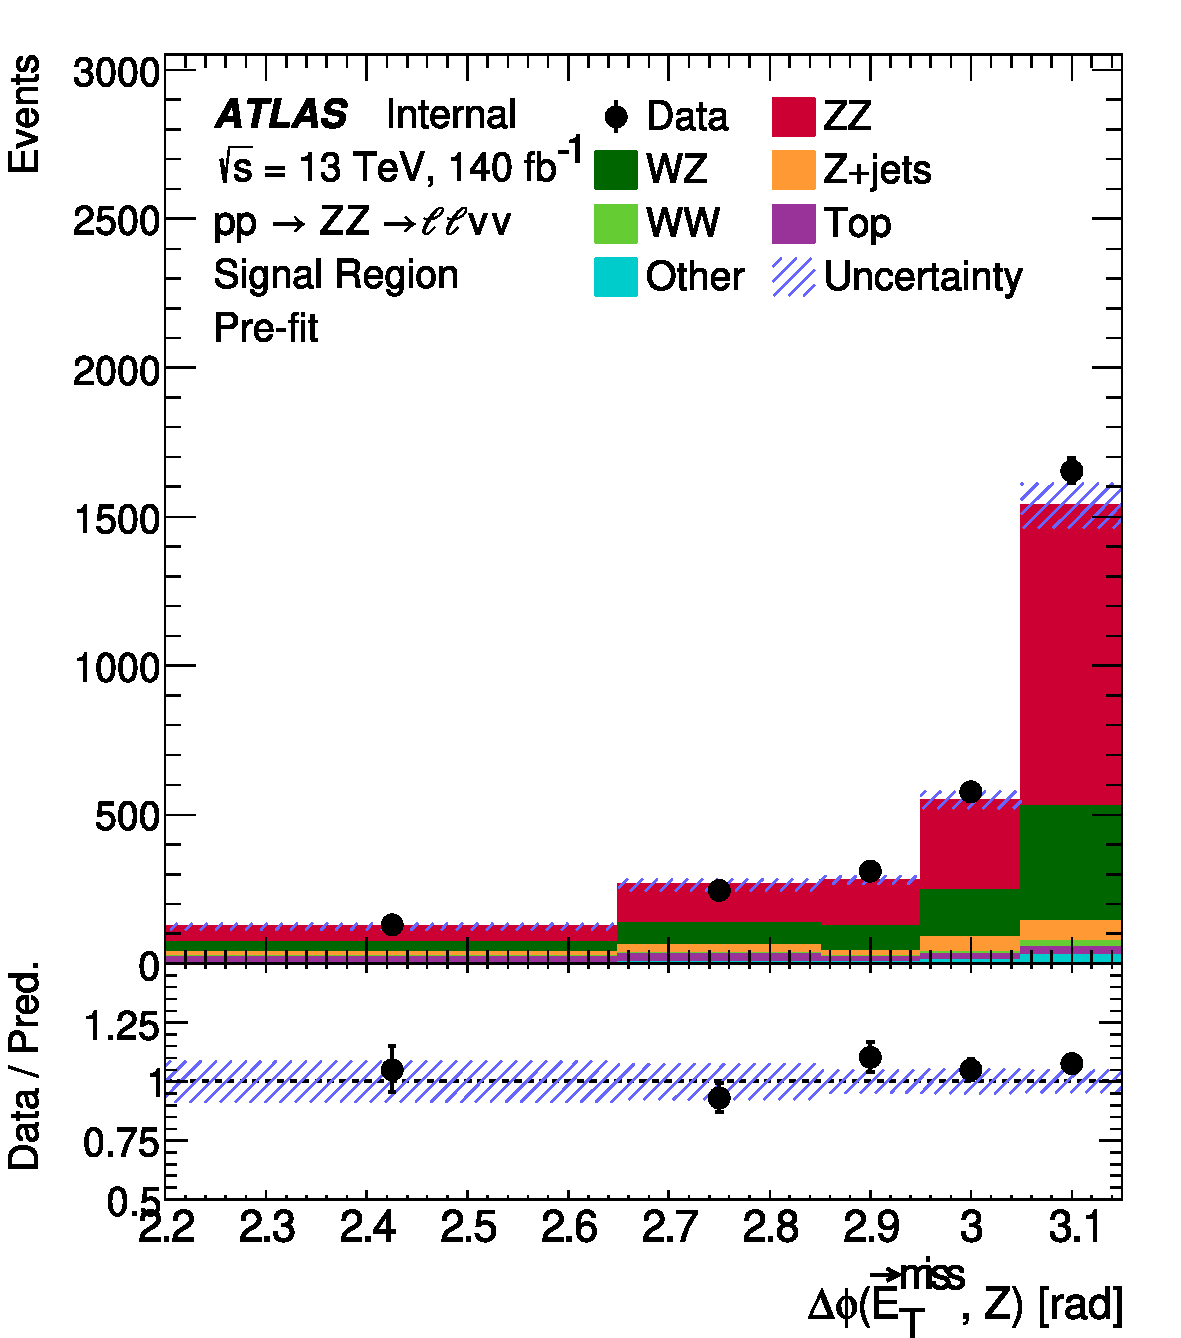
\includegraphics[width=0.45\linewidth]{figures/ch5-llvv/kin-distribution/SignalR-ZZ.pdf}}
    \vspace{0.5cm}
    \subfloat[]{   
    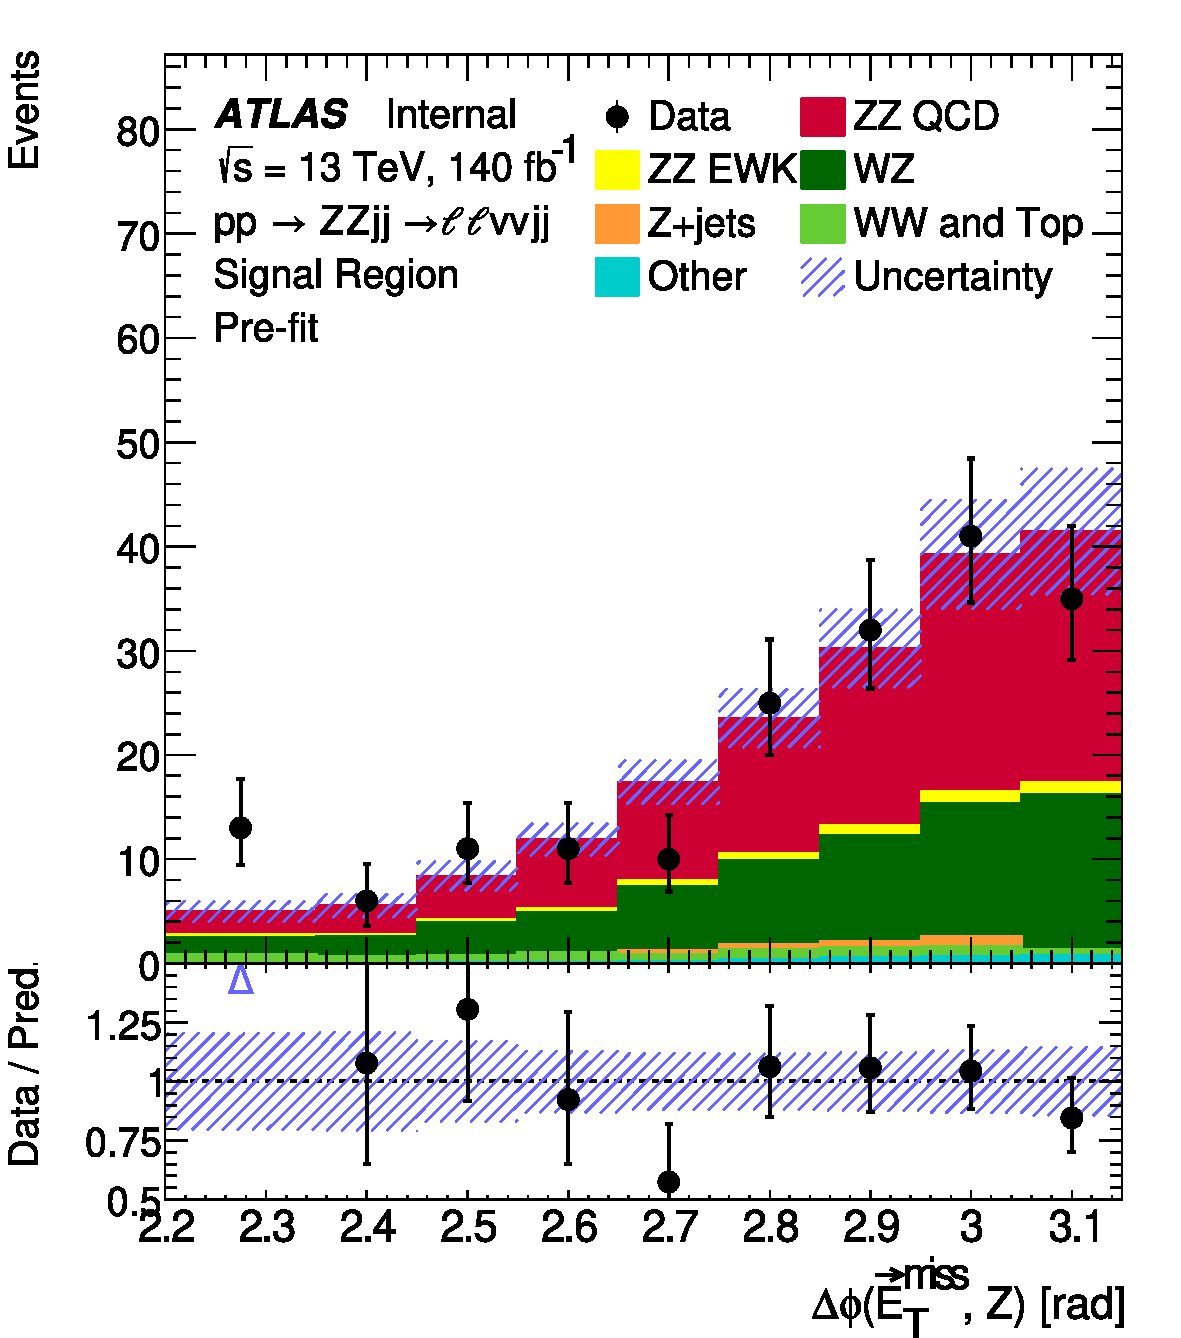
\includegraphics[width=0.45\linewidth]{figures/ch5-llvv/kin-distribution/SignalR-ZZjj.pdf}}
    \caption{Pre-fit comparative analysis between MC predictions and raw data mapping the $\Delta\phi(\vec{E}_{\text{T}}^{\text{miss}}, \text{Z})$ geometry inside the signal regions (SRs): (a) The inclusive $\text{ZZ}$ SR, and (b) The VBS-like $\text{ZZ}jj$ SR.}
    \label{fig:SR-prefit}
\end{figure}

% ======================================================================

%this subsection shall include more comparison and meaning of reco and truth selections. 
\subsubsection{Fiducial Phase Space Definition}
\label{sec:fiducial_definition}

Deriving precise differential and overall cross-sections for $\text{ZZ}$ production represents the core ambition of this analysis. However, raw detector-level observations are inextricably tangled with the acceptance rates of the event filter, which are fundamentally bound by algorithmic efficiencies and the detector's physical geometry. To bypass these hardware biases and deliver data that is directly cross-compatible with pure theoretical frameworks, the entire measurement is locked within a strictly defined \textbf{fiducial phase space}.

Establishing this fiducial boundary serves a dual purpose. Initially, it enforces a model-independent baseline by trapping the measurement strictly within the detector's actual sensory range. This prevents the analysis from heavily leaning on theoretical models to blindly extrapolate data into blind spots, thereby stripping away massive layers of theoretical uncertainty. Concurrently, it sets the necessary mathematical stage for generating the correction factors needed to translate raw detector-level event counts into authentic particle-level collision statistics.

This fiducial territory is mathematically carved out using pure particle-level (``truth'') telemetry sourced from the MC event generators. While these boundaries deliberately shadow the logic of the reconstruction-level filters, they are purposely relaxed. This strategic buffer ensures that the tighter detector-level selection envelope is completely swallowed by the larger fiducial volume. Employing this nested geometry stabilizes the efficiency calculations by virtually eliminating erratic event migrations across the selection borders. Specifically, limits targeting the dilepton invariant mass and missing transverse momentum are notably loosened at the truth level.

\paragraph{\textbf{The MC Truth Object Definitions}}
Prior to mapping the fiducial phase space via particle-level (``truth'') filtering, the underlying MC truth objects are synthesized through the following logic:
\begin{itemize}
    \item \textbf{Dressed Leptons:} To mathematically correct for final-state QED radiation, the four-momenta belonging to any prompt photons located within a tight $\Delta R(\ell, \gamma) < 0.1$ radius of a prompt muon or electron are folded directly into the lepton's baseline four-momentum. This generates ``dressed'' leptons, effectively bridging the gap between theoretical particles and realistic electromagnetic calorimeter measurements.
    \item \textbf{Truth Neutrinos:} The absolute truth missing transverse momentum ($E_{\text{T}}^{\text{miss, truth}}$) is computed by extracting the vector sum magnitude from the combined transverse momenta of every prompt neutrino present in the event.
    \item \textbf{Truth Jets:} Utilizing the anti-$k_t$ algorithm restricted to an $R=0.4$ radius, truth jets are assembled by clustering all stable particles inhabiting the final state (explicitly ignoring all neutrinos and the previously formulated dressed leptons).
\end{itemize}

\paragraph{\textbf{Fiducial Selection for Inclusive Production}}
To map the fiducial volume for the inclusive $\text{ZZ} \to \ell\ell\nu\nu$ cross-section, the truth-level objects must satisfy the following boundaries:
\begin{itemize}
    \item Precisely two dressed leptons of the same-flavour and opposite-sign (SFOS), restricted to $|\eta^\ell| < 2.5$.
    \item Transverse momentum floors demanding $p_{\text{T}}^\ell > 20~\text{GeV}$ for the subleading lepton and $p_{\text{T}}^\ell > 30~\text{GeV}$ for the leading candidate.
    \item A dilepton invariant mass securely positioned within the $76 < m_{\ell\ell} < 106~\text{GeV}$ bracket.
    \item A truth missing transverse momentum vaulting above $E_{\text{T}}^{\text{miss, truth}} > 95~\text{GeV}$.
    \item A strict dilepton angular separation capped at $\Delta R(\ell,\ell) < 1.8$.
    \item A wide azimuthal gap dividing the missing momentum and the dilepton system, requiring $\Delta\Phi(\vec{p}_{\text{T}}^{\,\ell\ell}, \vec{E}_{\text{T}}^{\text{miss, truth}}) > 2.2$.
    \item A scalar ratio dividing the missing momentum by the total transverse momentum exceeding $E_{\text{T}}^{\text{miss, truth}} / H_{\text{T}}^{\text{truth}} > 0.65$.
\end{itemize}

\paragraph{\textbf{Fiducial Selection for VBS-like $\text{ZZ}jj$ Production}}
Targeting the specialized $\text{ZZ}jj \to \ell^+\ell^-\nu\bar{\nu} jj$ cross-section, the fiducial volume imports the inclusive parameters but superimposes strict requirements on hadronic topologies:
\begin{itemize}
    \item Every inclusive fiducial parameter remains active, with the singular exception of the truth missing transverse momentum, which is aggressively raised to $E_{\text{T}}^{\text{miss, truth}} > 130~\text{GeV}$.
    \item The event is mandated to contain a minimum of two truth jets hitting $p_{\text{T}} > 30~\text{GeV}$ within an $|\eta| < 4.5$ envelope.
\end{itemize}

\paragraph{\textbf{Comparison of Detector-Level and Particle-Level Selections}}
To explicitly highlight the geometric relationship separating the ultimate signal regions from their foundational fiducial volumes, Tables~\ref{tab:reco_truth_inclusive} and~\ref{tab:reco_truth_vbs} provide a direct, side-by-side criteria breakdown. The calculated relaxation of the particle-level boundaries—most noticeably across $E_{\text{T}}^{\text{miss}}$ and $m_{\ell\ell}$—is heavily emphasized. This architectural buffer guarantees that standard detector resolution fluctuations cannot artificially bump a large segment of valid signal events outside the fiducial volume, a scenario that would irreparably destabilize the efficiency algorithms.

\begin{table}[!htbp]
    \centering
    \renewcommand{\arraystretch}{1.3}
    \begin{tabular}{l|c|c}
        \hline \hline
        \textbf{Requirement} & \textbf{Detector-Level (Reco)} & \textbf{Particle-Level (Truth)} \\
        \hline
        Leptons & \multicolumn{2}{c}{Exactly 2 SFOS leptons} \\
        Lepton $p_{\text{T}}$ [GeV] & \multicolumn{2}{c}{$> 30$ (lead), $> 20$ (sublead)} \\
        Lepton $|\eta|$ & $< 2.5$ ($\mu$); $< 2.47$ ($e$) & $< 2.5$ ($e, \mu$) \\
        Electron $|\eta|$ Veto & \textbf{Veto $1.37 < |\eta| < 1.52$} & \textbf{Not Applied} \\
        Dilepton Mass ($m_{\ell\ell}$) [GeV] & $80 < m_{\ell\ell} < 100$ & \textbf{$76 < m_{\ell\ell} < 106$} \\
        \hline
        Missing $E_{\text{T}}$ ($E_{\text{T}}^{\text{miss}}$) [GeV] & $> 110$ & \textbf{$> 95$} \\
        Dilepton $\Delta R(\ell,\ell)$ & $< 1.8$ & $< 1.8$ \\
        $\Delta\Phi(\vec{p}_{\text{T}}^{\,\ell\ell}, \vec{E}_{\text{T}}^{\text{miss}})$ & $> 2.2$ & $> 2.2$ \\
        $E_{\text{T}}^{\text{miss}} / H_{\text{T}}$ & $> 0.65$ & $> 0.65$ \\
        \hline
        $b$-Jet Veto & \textbf{Required} & \textbf{Not Applied} \\
        \hline \hline
    \end{tabular}
    \caption{Direct cross-comparison mapping the selection criteria for the \textbf{Inclusive $\text{ZZ}$ Signal Region} at the detector-level (Reco) against its encompassing particle-level (Truth) fiducial volume. Critical deviations are highlighted in \textbf{bold}.}
    \label{tab:reco_truth_inclusive}    
\end{table}

\begin{table}[!htbp]
    \centering
    \renewcommand{\arraystretch}{1.3}
    \begin{tabular}{l|c|c}
        \hline \hline
        \textbf{Requirement} & \textbf{Detector-Level (Reco)} & \textbf{Particle-Level (Truth)} \\
        \hline
        Inclusive Selection Base & Applied & Applied \\
        \hline
        Missing $E_{\text{T}}$ ($E_{\text{T}}^{\text{miss}}$) [GeV] & $> 150$ & \textbf{$> 130$} \\
        Number of Jets ($p_{\text{T}} > 30~\text{GeV}$) & $\geq 2$ & $\geq 2$ \\
        Jet $|\eta|$ &   $< 4.5$ & \textbf{$< 4.5$} \\
        \hline \hline
    \end{tabular}
    \caption{Direct cross-comparison mapping the selection criteria for the \textbf{VBS-like $\text{ZZ}jj$ Signal Region} at the detector-level (Reco) against its encompassing particle-level (Truth) fiducial volume. Structural differences are highlighted in \textbf{bold}.}
    \label{tab:reco_truth_vbs}
\end{table}

The fiducial parameters established here lay the groundwork for extracting the global correction factor, $C$, which mathematically scales the raw detector-level event count into a pure particle-level fiducial yield. Extracted entirely from simulations, this scalar repairs the background-subtracted data by accounting for resolution-driven data migrations and inherent detector blind spots. Mathematically, it is expressed as the ratio comparing the simulated signal events that successfully navigate the rigorous reconstruction-level filter ($N_{\text{Sel}}^{\text{MC}}$) against the volume of simulated signal events that clear the broader particle-level fiducial filter ($N_{\text{fid}}^{\text{MC}}$):
%
\begin{equation}
C = \frac{N_{\text{sel}}^{\text{MC}}}{N_{\text{fid}}^{\text{MC}}} \, .
\end{equation}

Consequently, the definitive fiducial cross-section, $\sigma_{\text{fid}}$, is derived via:
%
\begin{equation}
\sigma_{\text{fid}} = \frac{N_{\text{obs}} - N_{\text{bkg}}}{\mathcal{L}} \cdot \frac{1}{C} \, ,
\end{equation}
%
where $\mathcal{L}$ represents the total integrated luminosity, $N_{\text{bkg}}$ stands for the calculated background noise, and $N_{\text{obs}}$ reflects the sheer number of observed events locked inside the signal region. This structural equation brilliantly isolates the purely hardware-dependent variables ($C$) away from the theory-heavy extrapolations attempting to model the absolute total phase space.

Following this calculation, the correction factor for this specific analysis is anchored at $C = 56.1\%$. This value is synthesized by dividing the final selected MC signal yield by the product of the target integrated luminosity ($140~\text{fb}^{-1}$) and the baseline fiducial cross-section modeled via \textsc{Matrix}.


